\hypertarget{__smat__comp_8c}{
\section{\_\-smat\_\-comp.c File Reference}
\label{__smat__comp_8c}\index{_smat_comp.c@{\_\-smat\_\-comp.c}}
}


\subsection{Detailed Description}
\begin{Desc}
\item[For internal use only.]
This file contains the implementation of the \hyperlink{group__dbprim__smat_ga10}{\_\-smat\_\-comp()} function, the comparison callback used by sparse matrices.\end{Desc}


Definition in file \hyperlink{__smat__comp_8c-source}{\_\-smat\_\-comp.c}.

{\tt \#include \char`\"{}dbprim.h\char`\"{}}\par
{\tt \#include \char`\"{}dbprim\_\-int.h\char`\"{}}\par


Include dependency graph for \_\-smat\_\-comp.c:\begin{figure}[H]
\begin{center}
\leavevmode
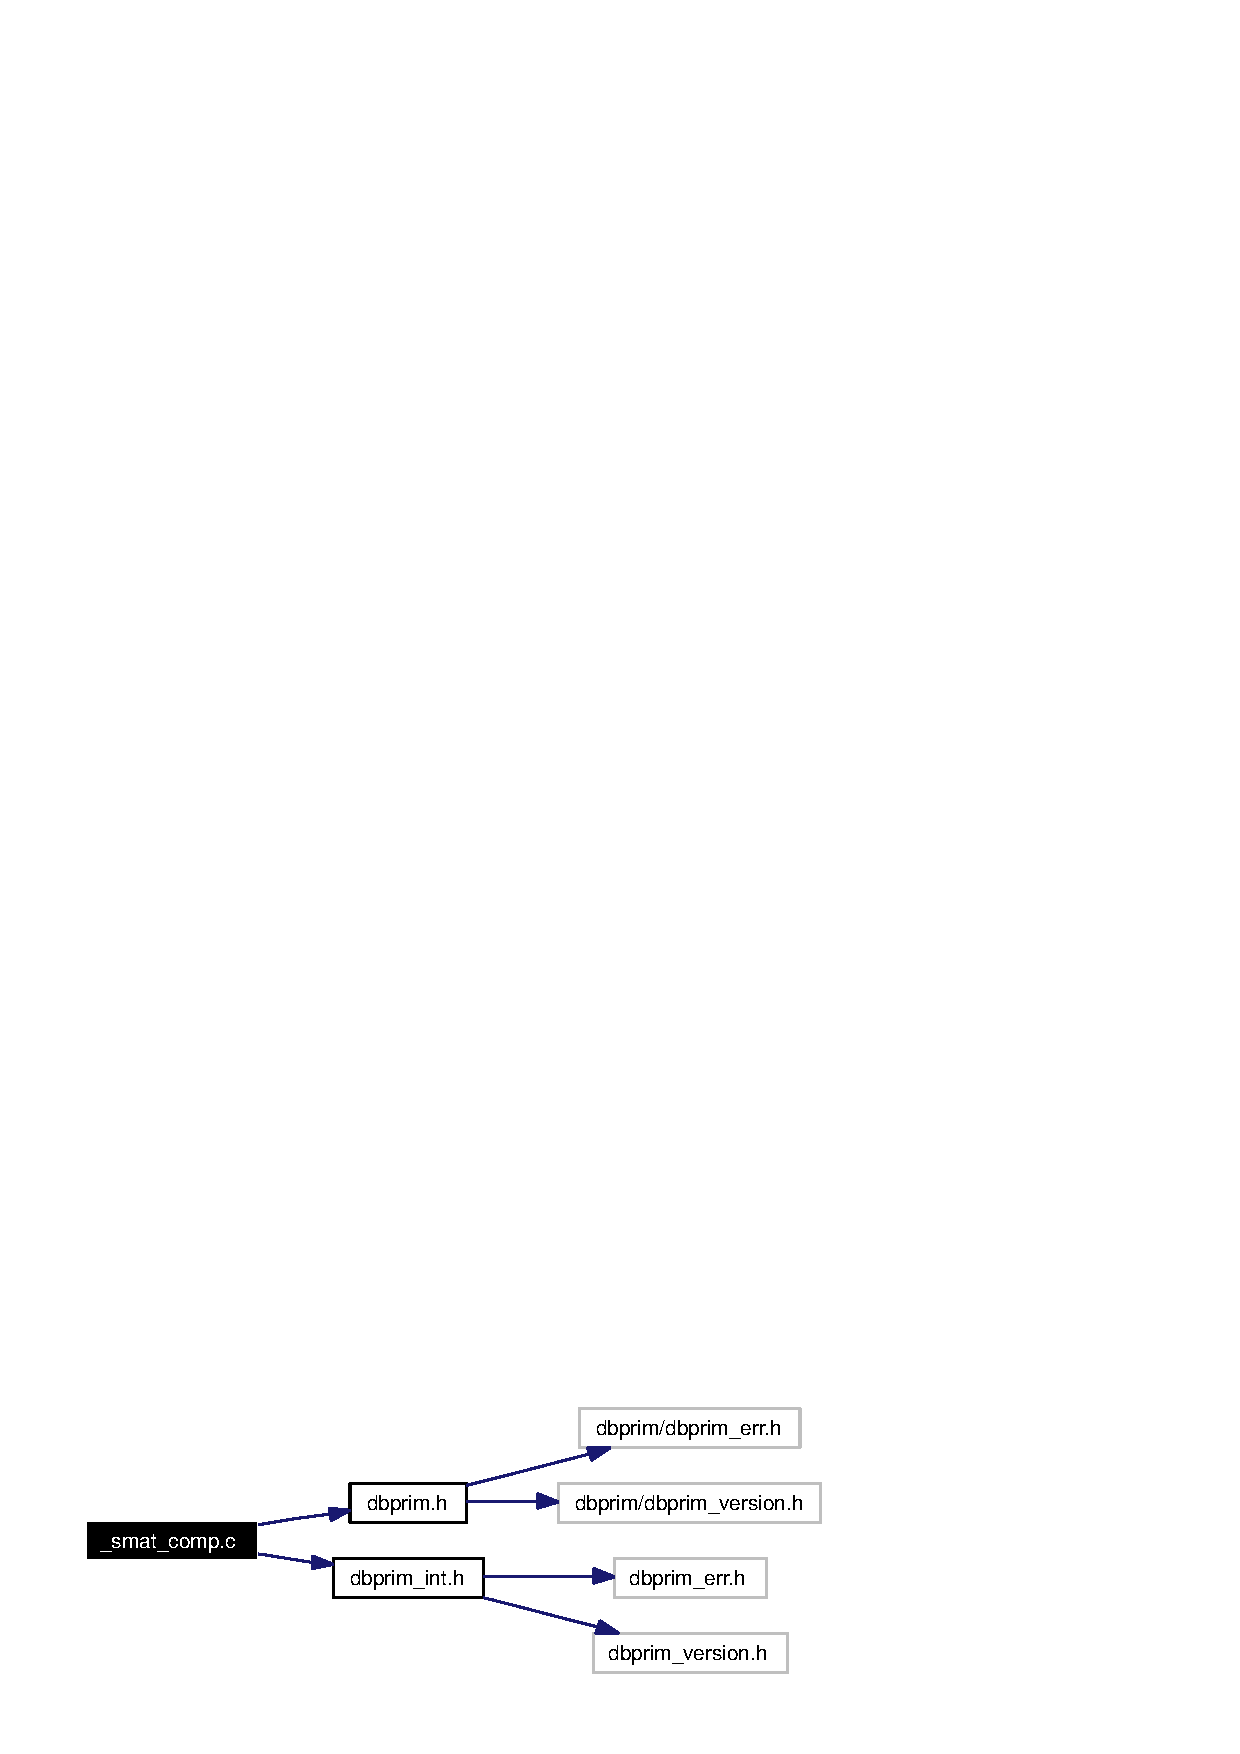
\includegraphics[width=199pt]{__smat__comp_8c__incl}
\end{center}
\end{figure}
\subsection*{Functions}
\begin{CompactItemize}
\item 
unsigned long \hyperlink{group__dbprim__smat_ga10}{\_\-smat\_\-comp} (\hyperlink{struct__hash__table__s}{hash\_\-table\_\-t} $\ast$table, \hyperlink{struct__db__key__s}{db\_\-key\_\-t} $\ast$key1, \hyperlink{struct__db__key__s}{db\_\-key\_\-t} $\ast$key2)
\begin{CompactList}\small\item\em Sparse matrix comparison function. \item\end{CompactList}\end{CompactItemize}
